\textbf{Por que a reconstrução não permite obter o sinal original?}

Do ponto de vista do sinal no domínio do tempo, a reconstrução do sinal é feita a partir de uma interpolação entre as amostras da sequência. Porém no caso da interpolação no domínio da frequência, ela pode ser representada pela filtragem passa-baixas para extrair uma única cópia do espectro periódico do sinal amostrado.

Porém uma filtragem passa-baixas ideal requer um filtro cuja resposta ao impulso é uma sinc, que não é executável na prática. O sinal sinc possui dois fatores limitantes para sua representação prática. Um fator limitante é que este sinal é não causal, ou seja, se estendendo para além do eixo negativo do tempo. Uma solução para a não causalidade é deslocar no tempo a resposta ao impulso do filtro. Porém isto resulta em outro problema, que é derivado da duração de uma sinc que é infinita. Como uma resposta ao impulso de duração infinita é impossível na prática, o projetista deve escolher em que ponto truncar a sinc, sendo que este ponto também está diretamente relacionado ao deslocamento no tempo que deve ser dado na sinc. Quanto mais períodos da sinc a resposta ao impulso do filtro possuir, mais fidedigna será a representação da sinc. Porém quanto mais períodos, maior será o deslocamento no tempo da resposta ao impulso para que se mantenha a simetria.

Dessa forma o sinal original não poderá ser perfeitamente recuperado após a reconstrução. A figura \ref{sincs} mostra um arranjo de diversas funções sincs organizadas em ordem de realizabilidade.

\begin{figure}[H] 
\centering
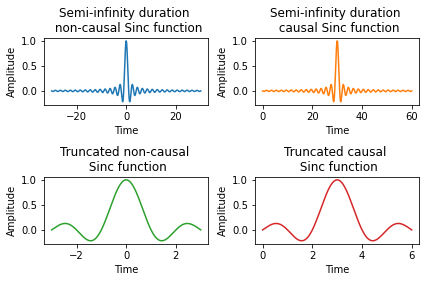
\includegraphics[width=13cm]{images/sincs.png}
\caption{Arranjo de funções sincs. Fonte: própria.}
\label{sincs} 
\end{figure}

De acordo com a figura \ref{sincs}, a sinc no canto superior esquerdo se aproxima do caso mais ideal possível, pois esta possui uma longa duração (porém o caso ideal seria infinito, por isso a escolha de palavras "duração semi-infinita"), mas ainda continua não causal. No canto superior direito há uma sinc de longa duração e causal, porém esta função como resposta ao impulso de um filtro de reconstrução introduziria um atraso semi-infinito no sinal de entrada, se mostrando assim inadequado. No canto inferior esquerdo há uma sinc que está truncada, resolvendo o problema de armazenar um filtro com uma grande quantidade de coeficientes, mas a não causalidade ainda continua. A última função sinc, no canto inferior direito, representa um caso realizável, pois está possui duração finita e é causal. Neste caso essa função como resposta ao impulso possuirá um pequeno número de coeficientes, introduzirá um pequeno atraso temporal, mas como está truncada não exercerá uma seletividade ideal, fazendo com que o filtro será tão seletivo quanto mais períodos da sinc estiverem truncados.

Falar do ROZ.